\documentclass[11pt,a4paper]{article}
\usepackage[margin=0.9in]{geometry}
\usepackage[T1]{fontenc}
\usepackage{lmodern}
\usepackage{amsmath,amssymb,amsthm}
\usepackage{graphicx}
\usepackage{microtype}
\usepackage{xcolor}
\usepackage[colorlinks=true,linkcolor=blue!55!black,citecolor=blue!55!black,urlcolor=blue!55!black]{hyperref}

\newtheorem{theorem}{Theorem}
\newtheorem{corollary}[theorem]{Corollary}
\newtheorem{remark}[theorem]{Remark}
\newcommand{\R}{\mathbb R}
\newcommand{\rhoR}[2]{\rho_{#1}(#2)}

\title{A $\Delta_2$-free sparse-transfer theorem\\
for the three-function Gagliardo--Nirenberg inequality}
\author{Autonomous mathematical discovery packet\\
Run \texttt{fa\_banach\_001}, lane 0, \texttt{agent\_lane\_00}}
\date{11 August 2026}

\begin{document}
\maketitle

\begin{center}
\fbox{\parbox{0.92\textwidth}{\textbf{Status.}
Substantial partial result, likely valid, pending human review.  The result
removes $\Delta_2$ in the source's full three-$N$-function regime for
Lebesgue measure and for an explicit sparse-transfer class of weights.  The
arbitrary nondoubling Hardy-weighted case remains open.}}
\end{center}

\section{The source question}

Ka\l amajska and Pietruska-Pa\l uba~\cite{KP} consider an $N$-function
$M$ and functions $P,Q$ satisfying
\begin{equation}\label{eq:Y}
 \frac{M(s)}{s^2}vw\le M(s)+P(v)+Q(w)
 \qquad(s,v,w>0).
\end{equation}
Under a Hardy inequality for $d\mu=e^{-\varphi}dx$, they prove a modular
estimate
\begin{equation}\label{eq:desired}
 \int_\Omega M(|\nabla u|)\,d\mu
 \le L\int_\Omega P(\theta|\nabla^2u|)\,d\mu
     +\int_\Omega Q(B|u|/\theta)\,d\mu
\end{equation}
for every $\theta>0$, and, when $P,Q$ are $N$-functions, its multiplicative
Luxemburg-norm consequence.  They ask whether the hypothesis
$M\in\Delta_2$ can be removed.

\begin{figure}[ht]
\centering

\includegraphics[width=0.96\textwidth]{figures/open_question_crop.png}
\caption{The explicit open question in arXiv:0910.5850, page 9.}
\end{figure}

The old proof needs $\Delta_2$ in an integration-by-parts estimate.  We
replace that step with the bounded-overlap sparse estimate of
Le\v{s}nik, Roskovec, and Soudsk\'y~\cite{LRS}.  Their Corollary 1.3 gives
constants $C_n,K_n>0$ such that for every $u\in C_c^2(\R^n)$ there is a
positive averaging operator
\[
 Tz=\sum_{A\in\mathcal A}\left(\frac1{|A|}\int_A z\right)\mathbf1_A,
 \qquad \sum_{A\in\mathcal A}\mathbf1_A\le K_n,
\]
for which
\begin{equation}\label{eq:sparse}
 |\nabla u|^2\le C_n\,T(|\nabla^2u|)\,T(|u|).
\end{equation}

\begin{figure}[ht]
\centering
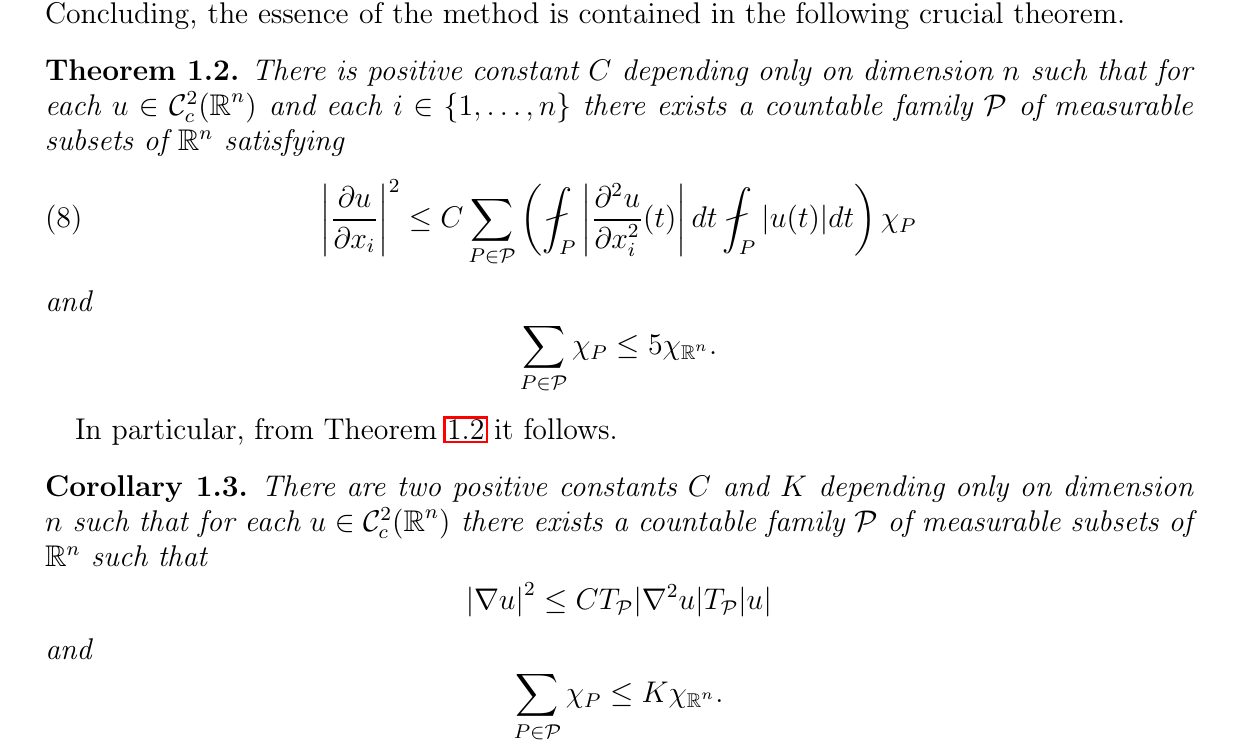
\includegraphics[width=0.88\textwidth]{figures/sparse_theorem_crop.png}
\caption{The sparse pointwise estimate and bounded-overlap property in
arXiv:2403.07096, page 4.}
\end{figure}

\section{The sparse-transfer theorem}

A \emph{Young function} below is finite, convex, nondecreasing, vanishes at
zero, and is not identically zero.  No doubling assumption is made.

\begin{theorem}[Lebesgue case]\label{thm:leb}
Let $\Omega\subset\R^n$ be open.  Let $M$ be an $N$-function, not
necessarily in $\Delta_2$, and let $P,Q$ be Young functions satisfying
\eqref{eq:Y}.  There is a constant
\[
 B_n=2C_nK_n^2,
\]
depending only on the dimension and the constants in \eqref{eq:sparse}, such
that every $u\in C_c^2(\Omega)$ and every $\theta>0$ satisfy
\begin{equation}\label{eq:main}
 \int_\Omega M(|\nabla u|)\,dx
 \le \int_\Omega P(\theta|\nabla^2u|)\,dx
     +\int_\Omega Q(B_n|u|/\theta)\,dx.
\end{equation}
If $P$ and $Q$ are $N$-functions, then
\begin{equation}\label{eq:norm}
 \|\nabla u\|_{L^M(\Omega)}
 \le 4\sqrt{B_n},
 \sqrt{\|\nabla^2u\|_{L^P(\Omega)}
       \|u\|_{L^Q(\Omega)}}.
\end{equation}
\end{theorem}

\begin{proof}
Extend $u$ by zero to $\R^n$ and take the operator $T$ in
\eqref{eq:sparse}.  Write
\[
 g=|\nabla u|,\qquad h=|\nabla^2u|,\qquad f=|u|,
 \qquad a=\frac{\theta}{K_n},\quad
 b=\frac{2C_nK_n}{\theta}.
\]
Thus $ab=2C_n$.  At a point where $g>0$, \eqref{eq:sparse} gives
$ab(Th)(Tf)\ge2g^2$.  Apply \eqref{eq:Y} with
$s=g$, $v=aTh$, and $w=bTf$:
\[
 M(g)
 \le \frac12\frac{M(g)}{g^2}(aTh)(bTf)
 \le \frac12\{M(g)+P(aTh)+Q(bTf)\}.
\]
After absorbing $M(g)/2$, this becomes
\begin{equation}\label{eq:point}
 M(g)\le P(aTh)+Q(bTf).
\end{equation}
The claim is automatic where $g=0$.

For every Young function $R$ and nonnegative $z$, bounded overlap and two
applications of Jensen's inequality give
\begin{equation}\label{eq:contract}
 \int_{\R^n}R(Tz/K_n)\,dx\le\int_{\R^n}R(z)\,dx.
\end{equation}
Indeed, at each point the at most $K_n$ averaging terms, supplemented by
zeros, form a convex combination; integration then counts every set at most
$K_n$ times.  Apply \eqref{eq:contract} first to
$R=P,z=\theta h$ and then to $R=Q,z=B_nf/\theta$.  Since
\[
 aTh=T(\theta h)/K_n,\qquad
 bTf=T(B_nf/\theta)/K_n,
\]
integrating \eqref{eq:point} proves \eqref{eq:main}.

For the norm assertion, put
$H=\|\nabla^2u\|_{L^P}$ and $U=\|u\|_{L^Q}$.  Assuming $H,U>0$, apply
\eqref{eq:main} to
\[
 \widetilde u=\frac{u}{\theta H+B_nU/\theta}.
\]
The defining modular property of the Luxemburg norm and monotonicity give
$\rho_M(\nabla\widetilde u)\le2$.  Convexity of $M$ then gives
$\rho_M(\nabla\widetilde u/2)\le1$, hence
\[
 \|\nabla u\|_{L^M}
 \le2\left(\theta H+\frac{B_n}{\theta}U\right).
\]
Minimizing over $\theta>0$ proves \eqref{eq:norm}.  The cases $H=0$ or
$U=0$ follow by the usual limiting argument (and give $\nabla u=0$).
\end{proof}

The proof isolates the exact weighted input it needs.

\begin{theorem}[Modular sparse transfer]\label{thm:transfer}
Let $d\mu$ be a measure on $\R^n$.  Suppose that every sparse operator $T$
arising in \eqref{eq:sparse} satisfies, for fixed $S_P,S_Q<\infty$,
\begin{equation}\label{eq:transfer}
 \int P(Tz/S_P)\,d\mu\le\int P(z)\,d\mu,
 \qquad
 \int Q(Tz/S_Q)\,d\mu\le\int Q(z)\,d\mu
\end{equation}
for all nonnegative $z$.  Then \eqref{eq:desired} holds with
$L=1$ and $B=2C_nS_PS_Q$, without any $\Delta_2$ assumption on $M$.
If $P,Q$ are $N$-functions, the corresponding norm estimate holds with
constant $4\sqrt{2C_nS_PS_Q}$.
\end{theorem}

\begin{proof}
Repeat the preceding proof with
$a=\theta/S_P$ and $b=2C_nS_P/\theta$.  Their product is $2C_n$;
\eqref{eq:point} is unchanged, and \eqref{eq:transfer} sends the two terms to
$P(\theta h)$ and $Q(2C_nS_PS_Qf/\theta)$.
\end{proof}

\begin{corollary}[Globally comparable densities]\label{cor:density}
Let $\Omega\subset\R^n$ be open and $d\mu=w(x)dx$, where
$0<m\le w\le W<\infty$ almost everywhere.  Put $\kappa=W/m$.
Under the hypotheses of Theorem~\ref{thm:leb}, both \eqref{eq:desired} and
its norm consequence hold without $\Delta_2$, with
\[
 L=1,\qquad B=2C_nK_n^2\kappa^2.
\]
\end{corollary}

\begin{proof}
Extend $w$ outside $\Omega$ while retaining the same bounds.  For every Young
function $R$, convexity, \eqref{eq:contract}, and $\kappa=W/m$ give
\[
 \int R\!\left(\frac{Tz}{\kappa K_n}\right)w,dx
 \le W\int R\!\left(\frac{T(z/\kappa)}{K_n}\right)dx
 \le \kappa\int R(z/\kappa)w,dx
 \le \int R(z)w,dx.
\]
Thus Theorem~\ref{thm:transfer} applies with
$S_P=S_Q=\kappa K_n$.
\end{proof}

\section{Scope and remaining obstruction}

Theorem~\ref{thm:leb} covers every $N$-function triple used for the source's
norm conclusion and keeps its general Young relation \eqref{eq:Y}; it is not
restricted to $P=Q=M$ or to inverse-function identities.  For the source's
modular-only conclusion, however, it adds convexity of $P,Q$, whereas the
source permits merely measurable nondecreasing functions.

More importantly, the Hardy hypothesis in~\cite{KP} controls the single
multiplier $|\nabla\varphi|$ in the $P$-modular.  It does not visibly imply
the two uniform sparse modular estimates \eqref{eq:transfer}, one of which is
needed in the $Q$-modular.  The paper's power and power--exponential examples
can have unbounded density oscillation, so Corollary~\ref{cor:density} does
not cover them.  Eight focused upgrade attempts included truncation of $M$,
high-elasticity counterexample families, weighted sparse averaging, and a
Hardy-to-sparse implication.  No proof or counterexample for arbitrary
nondoubling Hardy weights was obtained.

A bounded literature search through 11 August 2026 found no statement of the
three-function absorption theorem above.  The sparse estimate and its
one-function modular contraction are from~\cite{LRS}; their combination with
\eqref{eq:Y}, including the exact absorption and weighted transfer criterion,
is the new step claimed here.

\begin{thebibliography}{9}
\bibitem{KP}
A. Ka\l amajska and K. Pietruska-Pa\l uba,
\emph{On a variant of Gagliardo--Nirenberg inequality deduced from Hardy},
Bull. Pol. Acad. Sci. Math. 59 (2011), 133--149; arXiv:0910.5850.

\bibitem{LRS}
K. Le\v{s}nik, T. Roskovec, and F. Soudsk\'y,
\emph{Gagliardo--Nirenberg inequality via a new pointwise estimate},
arXiv:2403.07096 (2024), especially Theorem 1.2, Corollary 1.3, and the
modular observation in Section 4.
\end{thebibliography}

\end{document}
